\chapter{Introdu\c{c}\~ao e teoria}
%Estimação de estados 
%exemplo na pagina 16 do slide semana 7 
%Abordar método dos mínimos quadrados
%livro do monticelli - pag 268 - 




%\section{Motiva\c{c}\~ao}

% DIZER ALGO SOBRE COMO SERA O SISTEMA, COM BARRAS E CONEXOES E QUE FICA COMPLEXO SEM ANALISE DE FLUXO DE CARGA Mas como \'e possivel garantir o planejamento e opera\c{c}\~ao sistema de grandes propor\c{c}\~oes como esse? Para isso, \'e preciso saber o estado atual do sistema. Por\'em, n\~ao \'e vi\'avel medir todos os pontos de interesse. Isso seria custoso e tomaria muito tempo. 


%Para  como um todo \'e necessario que tenhamos ferramentas que nos ajudem a estimar o estado da rede 

%\section{Introdução à Teoria}
A ferramenta de an\'alise de sistemas de energia el\'etrica aqui discutida ser\'a a Estimação de Estado. Essa an\'alise nos fornecer\'a um metodo de obter o estado mais provável do sistema (ou de parte dele) a partir de medidas realizadas e a partir do modelo (circuito equivalente) da rede. \cite{monticelli}.
\section{Modelagem}
\label{SectionIntro}
%texto que explica como funciona
Para estimar o estado, será utilizado um conjunto de medidas que há disponível. Todas as redes de energia elétrica são constantemente monitoradas e, como toda medida, há uma incenteza atrelada, podendo ser erros aceitáveis e inaceitáveis (erros grosseiros).\\
É necessário que haja número de medidas em quantidade suficiente, para minimizar a influência dos erros grosseiros. Aliás, na hipótese de haver redundância no conjunto de medidas, é possível tratar erros nas medidas, já que pode-se lançar mão de ferramentas estatísticas.\\
Frequentemente, os valores calculados com o estado estimado, são mais confiáveis que o conjunto de medidas. \\
O modelo da rede e composto basicamente pelos circuitos equivalentes das linhas, transformadores, reguladores de tensão e por um gerador que proverá a referência angular da rede. Dispositivos de chaveamento e geradores distribuídos também podem ser modelados.\\
A topologia da rede e determinada pelo Configurador Topológico, que deve ser executado a cada alteração na topologia da rede.\cite{castro}

%formulas usadas no código
\section{Formula\c{c}\~ao do problema b\'asico}
\subsection{Mínimos Quadrados Ponderado}
Será utilizado modelos que descrevem as medições e suas relações, como em \ref{EQ_Modelo}

\begin{equation}
    z = \left[ 
    \begin{matrix} 
        z_1 \\
        z_2 \\
        \vdots \\
        z_m
    \end{matrix} \right]=\left[ 
    \begin{matrix} 
        h_1(x_1,x_2,...,x_n) \\
        h_2(x_1,x_2,...,x_n) \\
        \vdots \\
        h_m(x_1,x_2,...,x_n)
    \end{matrix} \right]+\left[ 
    \begin{matrix} 
        e_1 \\
        e_2 \\
        \vdots \\
        e_m
    \end{matrix} \right] = h(x) + e
    \label{EQ_Modelo}
\end{equation}
Onde $h_i(x)$ é a função que correlaciona a i-ésima medição com o vetor de estado, $x^t = [x_1, x_2,\hdots, x_n ]$ é o vetor de estado que contém as n variáveis de estado e $e^t = [e_1, e_2,\hdots, e_m ]$ corresponde ao vetor de erros do processo de medição.\\
Os elementos de $e$ possuem média nula, $E\{e_i e_i\} = 0$, e $Cov(e) = E[e.e^t] = R_z = diag\{\sigma_1^2, \sigma_2^2, \hdots, \sigma_m^2\}$. A variância $\sigma_i^2$ é calculada de acordo com a precisão da medição.\\
No método dos mínimos quadrados ponderados a função \ref{EQ_Jacobiana} deve ser minimizada. O inverso do desvio padrão é usado na ponderação das medidas. \cite{castro}
\begin{equation}
    J(x) = \sum_{i=1}^{m} \frac{(z_i - h_i(x))^2}{\sigma_i^2} = [z-h(x)]'R_z^-1[z-h(x)]
    \label{EQ_Jacobiana}
\end{equation}
\subsection{Equação normal}
\label{SectionFormula}
Ao minimizar a equação \ref{EQ_Jacobiana}, é necessário derivá-la e igualar a zero. Como resultado, o estado estimado é obtido iterativamente com método dos minimos quadrados ponderados, conforme a equação \ref{WLS_G}.
\begin{equation}
    G(x^\nu). \Delta x^\nu = H'(x^\nu).R_z^-1 [z-H(x^\nu)]
    \label{WLS_G}
\end{equation}
E,
\begin{equation}
    x^{\nu+1} = x^\nu + \Delta x^\nu
\end{equation}
A matriz Hessiana $G(x)$, chamada de matriz Ganho, é definida como em \ref{G}
\begin{equation}
    G(x) = H'(x)R_z^{-1}H(x)
    \label{G}
\end{equation}
O uso da matriz $G$, de ganhos, é conhecido como solução via equação normal e esta solução apresenta boa convergênca. Em alguns casos, porém, a solução da equação \ref{WLS_G} pode apresentar divergência (não será abordado neste trabalho).\\
A formação da matriz $H$, descrita em \ref{G}, é dada por \ref{H}.
\begin{figure}[!htb]
\caption{Formulação da matriz $H$}
 \centering % para centralizarmos a figura
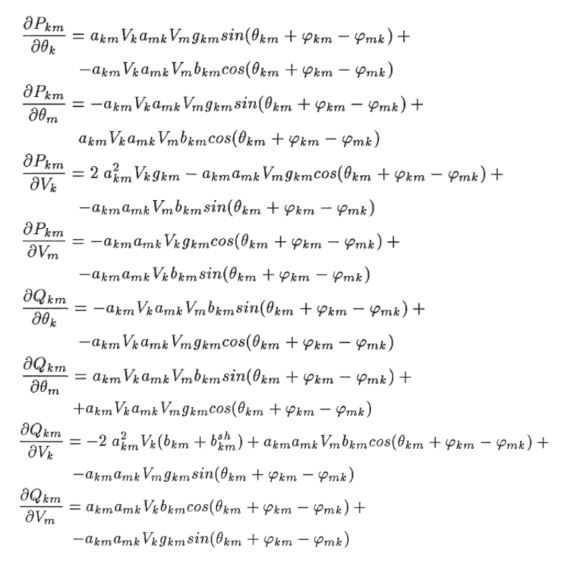
\includegraphics[width=12cm]{figuras/H.JPG}
\label{H}
\end{figure}
\subsection{Tableau Esparso}
Para evitar trabalhar com o produto de H (matriz G), como em \ref{G}, pode-se reescrever o problema como minimização com restrições, como em \ref{EQ_minJ} e \ref{EQ_minJ2}
\begin{equation}
    minJ(x) = \frac{1}{2}[z-h(x)]R_z^{-1} [z-h(x)]
    \label{EQ_minJ}
\end{equation}
\begin{equation}
    minJ(x) = \frac{1}{2}r'R_z^{-1}r
    \label{EQ_minJ2}
\end{equation}
Sujeito a $r = z-h(x)$. 
Para resolver este problema, deve-se usar multiplicadores de Lagrange. A solução pode ser obtida iterativamente a partir de \ref{EQ_Tableau}.
\begin{equation}
    \left[ 
    \begin{matrix} 
        R_z & H(x^k) \\
        H'(x^k) & 0
    \end{matrix} \right] \left( 
    \begin{matrix} 
        \lambda^k \\
        \Delta x^k
    \end{matrix} \right) = \left[ 
    \begin{matrix} 
        z-h(x^k) \\
        0
    \end{matrix} \right]= \left[ 
    \begin{matrix} 
        \Delta z(x^k) \\
        0
    \end{matrix} \right]
    \label{EQ_Tableau}
\end{equation}
Neste processo, há a matriz $H$ e não a matriz $G$, o que melhora o condicionamento da matriz a ser fatorada. \cite{castro}. 

%%%%%%%%%%%%%%%%%%%
\section{Algoritmo implementado}
Basicamente, tem-se 4 etapas do processo de estimação de estado \cite{Mohamad}. 
\begin{enumerate}
    \item Processamento da topologia. Todas as informações de representação da topologia são tratadas.
    \item Analise de observabilidade. A partir do modelo barra-ramo obtido na primeira etapa, verifica-se se é possivel determinar as tensões e angulos em todas as barras, considerando as medidas disponíveis.
    \item Estimação de estado. A partir da topologia, dos parâmetros e dos conjuntos de medidas disponíveis, o Estimador de Estado determina a estimação que melhor representa o sistema
    \item Processamento de erros grosseiros. A presença de medidas analógicas com possibilidade de erros grosseiros afasta a solução verdadeira do estimador de estados. Se uma medida é identificada dessa forma, ela deve ser retirada da solução. 
    
\end{enumerate}

